%\section{Практична реалізація}
\section{ПРАКТИЧНА РЕАЛІЗАЦІЯ}

Даний розділ присвячується аналізу роботи алгоритмів Deep InfoMax та Momentum Contrast.

\subsection{Технології, використані у ДР}

Python $-$ це легка в освоєнні, потужна мова програмування. Він має ефективні структури даних високого рівня і простий, але ефективний підхід до об'єктно-орієнтованого програмування [7].

Python став загальноприйнятою мовою програмування для багатьох сфер застосування науки про дані. Дана мова програмування поєднує в собі міць мов програмування з простотою використання предметно орієнтованих скриптових мов типу MATLAB або R. 

В Python є бібліотеки для завантаження даних, візуалізації, статистичних обчислень, обробки природної мови, обробки зображень і багато чого іншого [8].

Також використовувався фреймфорк Anaconda. Це безкоштовний, включаючи комерційне використання, і готовий до використання в середовищі підприємства дистрибутив Python, який об'єднує всі ключові бібліотеки Python, необхідні для роботи в області науки про дані, математики та розробки, в одному зручному для користувача крос-платформенном дистрибутиві [9].

Для тренування нейронних мереж було обрано бібліотеку PyTorch. PyTorch - це бібліотека для програм Python, яка сприяє побудові проектів глибокого навчання [10].

Також використовувалась бібліотеки NumPy та matplotlib. NumPy є основним пакетом для наукових обчислень з Python [11]. Matplotlib $-$ це всебічна бібліотека для створення статичних, анімованих та інтерактивних візуалізацій у Python [12]. 

%\vspace{1em}
\newpage

\subsection{Дані для аналізу}

Для демонстрації та аналізу роботи алгоритмів були використані дані з датасету CIFAR-10.

Набір даних CIFAR-10 складається з 60000 кольорових зображень розміром 32x32 у 10 класах, по 6000 зображень на клас. Існує 50000 навчальних зображень та 10000 тестових зображень [13].

Набір даних розділений на п’ять навчальних партій та одну тестову партію, кожна з 10000 зображень. Тестова партія містить рівно 1000 довільно обраних зображень з кожного класу. Навчальні партії містять решту зображень у довільному порядку, але деякі навчальні партії можуть містити більше зображень одного класу, ніж інші [13]. Навчальні партії містять рівно 5000 зображень від кожного класу.

Приклад зображень з датасету наведено у рис. \ref{fig:cifar10}.

\vspace{1em}

\begin{figure}[h]
  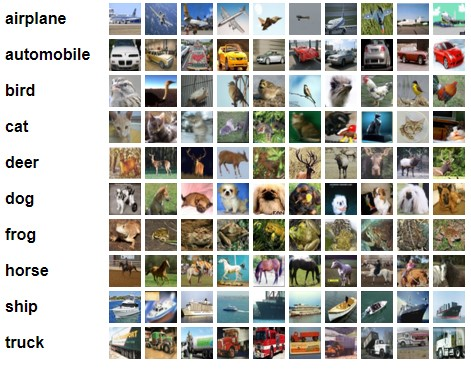
\includegraphics[width=\textwidth, height=8cm, natwidth=471, natheight=370]{cifar10.jpg}
  \caption{Зображення з датасету CIFAR-10}
  \label{fig:cifar10}
\end{figure}

\subsection{Аналіз роботи алгоритму Deep InfoMax}

Робота методу Deep InfoMax буде розглядатись в залежності від значень гіперпараметрів $\alpha$, $\beta$ та $\gamma$, а також коефіціенту швидкості навчання. В кожному експерименті кількість епох навчання нейронної мережі складатиме 300.

Якщо взяти $\alpha = 0,1$, $\beta = 0,1$ та $\gamma = 0,1$, то помилка на тренувальних даних буде 12,73 \% та модель тренувалась приблизно 14 годин.

На рис. \ref{fig:deepinfodemo1} можна побачити, що модель доволі погано узагальнює результати.

\vspace{1em}
%\newpage

\begin{figure}[h]
  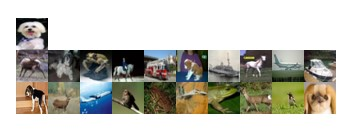
\includegraphics[width=\textwidth, height=5cm, natwidth=345, natheight=130]{deepinfodemo1.jpg}
  \caption{Результати тестування при $\alpha = 0,1; \, \beta = 0,1; \, \gamma = 0,1$}
  \label{fig:deepinfodemo1}
\end{figure}

У таблиці \ref{tab:deepinfoerror} представлено результати тестування при різних гіперпараметрах:

\begin{table}[h]
\caption{Залежність роботи моделі від $\alpha$, $\beta$ та $\gamma$}\label{tab:deepinfoerror}
\begin{tabular}{|m{0.15\textwidth}|m{0.15\textwidth}|m{0.15\textwidth}|m{0.2\textwidth}|m{0.2\textwidth}|}
\hline
$\alpha$ & $\beta$ & $\gamma$ & Помилка \% & Час год. \\
\hlinewd{2pt}
	0,1 & 0,1 & 0,1 & 12.73 & 14 \\
\hline
	0,3 & 0,3 & 0,3 & 14,88 & 12 \\
\hline
	0,5 & 0,5 & 0,5 & 7,56 & 11 \\
\hline
	0,5 & 0,1 & 0,3 & 8,34 & 12 \\
\hline
	0,6 & 0,6 & 0,6 & 4,43 & 9 \\
\hline
	0,6 & 0,1 & 0,3 & 6,74 & 9 \\
\hline
	0,7 & 0,7 & 0,7 & 3,98 & 8 \\
\hline
	0,7 & 1 & 0,7 & 5,22 & 9 \\
\hline
	0,7 & 1 & 0,3 & 6,72 & 8 \\
\hline
	0,7 & 1 & 0,1 & 3,16 & 7 \\ 
\hline
	0,5 & 0,7 & 0,1 & 2,57 & 6 \\
\hline
	0,5 & 0,9 & 0,1 & 1,28 & 6 \\
\hline
	0,5 & 1 & 0,1 & 1,45 & 6 \\
\hline
\end{tabular}
\end{table}


Як можна спостерігати, найменша помилка отримується при $\alpha = 0,5$, $\beta = 0,9$ та $\gamma = 0,1$. Результати тестування можна побачити на рис. \ref{fig:deepinfodemo2}. Помилка на тестувальних даних складала 36,96 \%.

\vspace{1em}

\begin{figure}[h]
  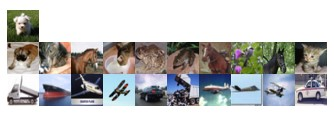
\includegraphics[width=\textwidth, height=5cm, natwidth=334, natheight=114]{deepinfodemo2.jpg}
  \caption{Результати тестування при $\alpha = 0,5; \, \beta = 0,9; \, \gamma = 0,1$}
  \label{fig:deepinfodemo2}
\end{figure}

Дані результати були отримані за умови, що коефіцінет швидкості навчання дорівнював 0,001. На рис. \ref{fig:deepinfolearning} представлено залежність якості тренування від значень даного параметру.

\begin{figure}[h]
  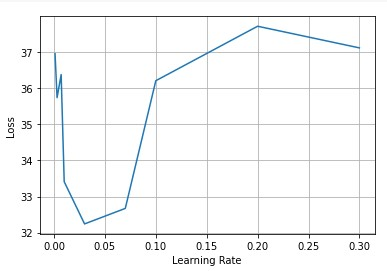
\includegraphics[width=\textwidth, height=8cm, natwidth=387, natheight=271]{deepinfolearning.jpg}
  \caption{Залежність якості тренування від коефіціенту швидкості навчання}
  \label{fig:deepinfolearning}
\end{figure}

З рис. \ref{fig:deepinfolearning} видно, що найкращі результати отримуються при коефіціенті 0,03. На рис. \ref{fig:deepinfodemo3} можна бачити результати тестування. Помилка в такому випадку складає 32,24 \%та час тренування $-$ приблизно п'ять годин.

\newpage

\begin{figure}[h]
  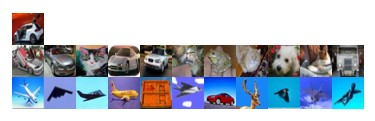
\includegraphics[width=\textwidth, height=5cm, natwidth=375, natheight=121]{deepinfodemo3.jpg}
  \caption{Результати тестування при оптимальних параметрах}
  \label{fig:deepinfodemo3}
\end{figure}

\subsection{Аналіз роботи алгоритму Momentum Contrast}

Робота методу Momentum Contrast буде розглядатись в залежності від значень гіперпараметру $\tau$, та коефіціенту швидкості навчання. В кожному експерименті кількість епох навчання нейронної мережі складатиме 300.

Якщо взяти $\tau = 0,01$, то помилка на тренувальних даних буде складати 17,64 \% та модель тренувалась приблизно дев'ять годин.

На рис. \ref{fig:mocodemo1} можна побачити, що модель доволі погано узагальнює результати.

\vspace{1em}
%\newpage

\begin{figure}[h]
  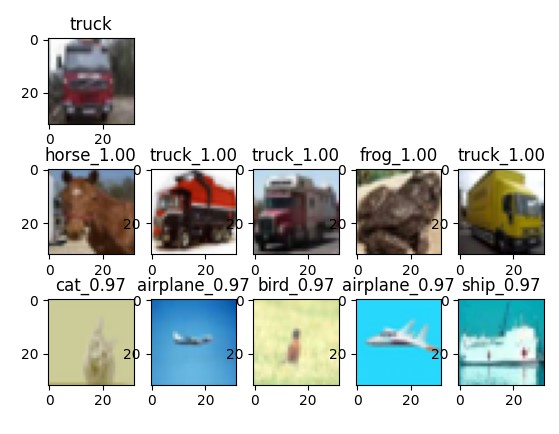
\includegraphics[width=\textwidth, height=9cm, natwidth=559, natheight=434]{mocodemo1.jpg}
  \caption{Результати тестування при $\tau = 0,01$}
  \label{fig:mocodemo1}
\end{figure}

У таблиці \ref{tab:mocoerror} представлено результати тестування при різних гіперпараметрах:

\begin{table}[h]
\caption{Залежність роботи моделі від $\tau$}\label{tab:mocoerror}
\begin{tabular}{|m{0.15\textwidth}|m{0.2\textwidth}|m{0.2\textwidth}|}
\hline
$\tau$ & Помилка \% & Час год. \\
\hlinewd{2pt}
	0,01 & 17.64 & 9 \\
\hline
	0,03 & 15,69 & 8 \\
\hline
	0,05 & 14,97 & 8 \\
\hline
	0,07 & 12,66 & 7 \\
\hline
	0,1 & 8,73 & 6 \\
\hline
	0,3 & 7,43 & 5 \\
\hline
	0,7 & 5,71 & 4 \\
\hline
	0,9 & 6,38 & 4 \\
\hline
\end{tabular}
\end{table}


Як можна спостерігати, найменша помилка отримується за умови $\tau = 0,7$. Результати тестування можна побачити на рис. \ref{fig:mocodemo2}. Помилка на тестувальних даних складала 40,34 \%.

%\newpage

\begin{figure}[h]
  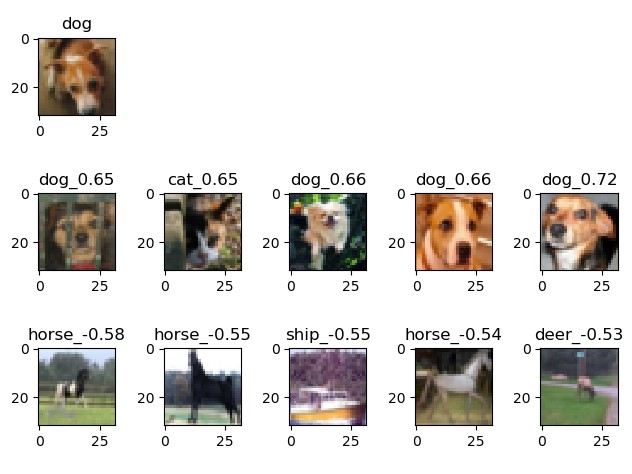
\includegraphics[width=\textwidth, height=9cm, natwidth=632, natheight=474]{mocodemo2.jpg}
  \caption{Результати тестування при $\tau = 0,7$}
  \label{fig:mocodemo2}
\end{figure}

Дані результати були отримані за умови, що коефіцінет швидкості навчання дорівнював 0,001. На рис. \ref{fig:mocolearning} представлено залежність якості тренування від значень даного параметру.

\begin{figure}[h]
  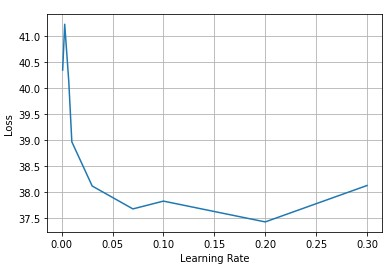
\includegraphics[width=\textwidth, height=8cm, natwidth=391, natheight=268]{mocolearning.jpg}
  \caption{Залежність якості тренування від коефіціенту швидкості навчання}
  \label{fig:mocolearning}
\end{figure}

%\newpage

З рис. \ref{fig:mocolearning} видно, що найкращі результати отримуються при коефіціенті 0,2. На рис. \ref{fig:mocodemo3} можна бачити результати тестування. Помилка в такому випадку складає 37,42 \% та час тренування $-$ приблизно чотири години.

%\newpage
\vspace{1em}

\begin{figure}[h!]
  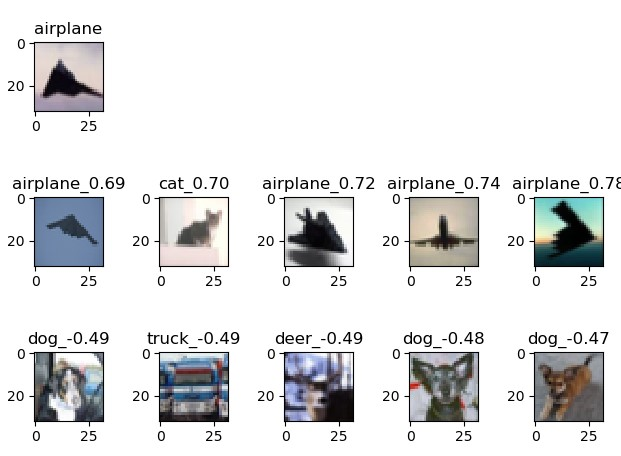
\includegraphics[width=\textwidth, height=8cm, natwidth=621, natheight=456]{mocodemo3.jpg}
  \caption{Результати тестування при оптимальних параметрах}
  \label{fig:mocodemo3}
\end{figure}

\newpage

\subsection{Висновки за розділом}

В даному розділі була продемонстрована робота алгоритмів Deep InfoMax та Momentum Contrast. Були реалізовані програми мовою програмування Python за допомогою спеціальних бібліотек для аналізу даних та програмного фреймворку Anaconda. 

Як видно з результатів, модель Deep InfoMax дає якісніший прогноз, в той час як алгоритм Momentum Contrast потребує менше часових та обчислювальних ресурсів.
